\documentclass[12pt,a4paper]{article}

% ── Packages ──────────────────────────────────────────────────────────────────
\usepackage[a4paper, top=2.5cm, bottom=2.5cm, left=2.8cm, right=2.8cm]{geometry}
\usepackage{amsmath, amssymb, amsthm}
\usepackage{mathtools}
\usepackage{xcolor}
\usepackage{tcolorbox}
\usepackage{fancyhdr}
\usepackage{graphicx}
\usepackage{tikz}
\usepackage{pgfplots}
\pgfplotsset{compat=1.18}
\usepackage{enumitem}
\usepackage{booktabs}
\usepackage{microtype}
\usepackage{parskip}
\usepackage{mdframed}
\usepackage{titlesec}
\usepackage{caption}
\usepackage{float}
\usepackage{array}
\usepackage{colortbl}
\usepackage{hyperref}

\usetikzlibrary{arrows.meta, decorations.markings, positioning,
                shapes.geometric, calc, patterns, backgrounds}

\geometry{top=2.5cm, bottom=2.5cm, left=2.8cm, right=2.8cm,
          headheight=15pt}

% ── Colours ───────────────────────────────────────────────────────────────────
\definecolor{deepblue}{RGB}{10,40,90}
\definecolor{midblue}{RGB}{30,80,160}
\definecolor{lightblue}{RGB}{220,235,255}
\definecolor{accentgold}{RGB}{180,140,20}
\definecolor{palegreen}{RGB}{230,248,235}
\definecolor{palegold}{RGB}{255,250,225}
\definecolor{brickred}{RGB}{160,30,30}

% ── Running header ────────────────────────────────────────────────────────────
\pagestyle{fancy}
\fancyhf{}
\renewcommand{\headrulewidth}{0.4pt}
\fancyhead[L]{\large\bfseries\color{midblue} Josephite Math Club}
\fancyhead[R]{\includegraphics[height=10mm]{Screenshot 2026-02-04 154432.png}}

% ── Section formatting ────────────────────────────────────────────────────────
\titleformat{\section}{\large\bfseries}{\thesection.}{0.5em}{}
  [\vspace{0.15em}\hrule\vspace{0.3em}]
\titlespacing{\section}{0pt}{1.8em}{0.8em}

\titleformat{\subsection}
  {\normalsize\bfseries\color{midblue}}{\thesubsection.}{0.5em}{}

% ── tcolorbox styles ──────────────────────────────────────────────────────────
\tcbuselibrary{skins, breakable, theorems}

\newtcolorbox{definitionbox}[1]{
  colback=cyan!6, colframe=cyan!40!black,
  fonttitle=\bfseries\color{white},
  title={#1}, arc=4pt,
  left=6pt, right=6pt, top=4pt, bottom=4pt,
  breakable
}

\newtcolorbox{theorembox}[1]{
  colback=blue!5, colframe=blue!25!black,
  fonttitle=\bfseries\color{white},
  title={#1}, arc=4pt,
  left=6pt, right=6pt, top=4pt, bottom=4pt,
  breakable
}

\newtcolorbox{warningbox}[1]{
  colback=red!14, colframe=red!34!black,
  fonttitle=\bfseries\color{white},
  title={#1}, arc=4pt,
  left=6pt, right=6pt, top=4pt, bottom=4pt,
  breakable
}

\newtcolorbox{procedurebox}[1]{
  colback=gray!8, colframe=gray!60!black,
  fonttitle=\bfseries,
  title={#1}, arc=4pt,
  left=6pt, right=6pt, top=4pt, bottom=4pt,
  breakable
}

% ── Hyperref ──────────────────────────────────────────────────────────────────
\hypersetup{
  colorlinks=true,
  linkcolor=midblue,
  urlcolor=midblue,
  citecolor=midblue
}

% ── Example environment ───────────────────────────────────────────────────────
\newenvironment{example}[1]{%
  \vspace{0.8em}
  \noindent{\footnotesize\scshape\color{orange!50!black} Example}\par
  \noindent\textbf{#1}\par\vspace{0.3em}
  \begin{list}{}{\leftmargin=1em\rightmargin=0pt}\item
}{%
  \end{list}\vspace{0.8em}
}

% ── Custom commands ───────────────────────────────────────────────────────────
\newcommand{\R}{\mathbb{R}}
\newcommand{\C}{\mathbb{C}}
\newcommand{\ODE}{\textsc{ode}}
\newcommand{\ee}{\mathrm{e}}
\newcommand{\ii}{\mathrm{i}}
\newcommand{\dd}{\mathrm{d}}

\setlength{\parskip}{6pt}

% ── Insight plain (italic grey remark block) ──────────────────────────────────
\newenvironment{insight_plain}{%
  \vspace{0.4em}\begin{list}{}{\leftmargin=1em}\item\small\itshape\color{gray!70!black}%
}{\end{list}\vspace{0.4em}}

% ─────────────────────────────────────────────────────────────────────────────
\begin{document}

% ── Title page ────────────────────────────────────────────────────────────────
\begin{titlepage}
    \centering
    \vspace*{2cm}

\begin{center}
    \includegraphics[scale=0.4]{sjs x jmc .png}
\end{center}

    {\footnotesize\scshape Ordinary Differential Equations\enspace·\enspace
    Part 3}

    {\LARGE\bfseries Non-Homogeneous Linear ODEs: Driving the System\par}

    \vspace{1.5cm}

    {\large \scshape Asif Ahmed Tamim}

    \vspace{2.5cm}

    \begin{center}
\itshape
``A good notation has a subtlety and suggestiveness which at times make\\
it seem almost like a live teacher.''\\[4pt]
\upshape --- Bertrand Russell
    \end{center}

    \vspace*{\fill}
\end{titlepage}

% ─────────────────────────────────────────────────────────────────────────────
\section{Introduction}
% ─────────────────────────────────────────────────────────────────────────────

In Parts~1 and~2 we solved equations where the system was ``left alone'': first-order
equations governed entirely by the ratio $y/x$, and second-order linear equations
with zero on the right-hand side. Real physical systems, however, are rarely isolated.
A mass on a spring gets pushed. A circuit gets connected to a power supply. A bridge
gets buffeted by wind. An atom gets illuminated by a laser. In each case, the
governing ODE acquires a \emph{non-zero right-hand side} --- a \textbf{forcing
function}, or \textbf{driving term} --- that represents this external influence.

The equation we study in this part is
\begin{equation}
  y'' + P(x)\,y' + Q(x)\,y = R(x),
  \label{eq:nhom}
\end{equation}
where $R(x) \not\equiv 0$. This is called a \textbf{non-homogeneous linear ODE}. The
function $R(x)$ is variously called the forcing function, the input, the driving term,
or the source term. The homogeneous equation with $R = 0$, which we solved in
Part~2, is now called the \textbf{reduced equation} or the \textbf{complementary
equation} associated with \eqref{eq:nhom}.

The central theorem of this part reveals the beautifully structured form of every
solution: the \emph{general solution of the non-homogeneous equation} is always the
sum of the general solution of the complementary equation and any single
\emph{particular solution} of the full equation. This \textbf{complementary-plus-particular
structure} means we can split a complicated problem into two tractable pieces.

We will develop two systematic methods for finding particular solutions. The first,
\textbf{undetermined coefficients}, is fast and elegant but works only when $R(x)$ has
a special form. The second, \textbf{variation of parameters}, is completely general: it
works for any continuous $R(x)$, at the cost of some integration. We apply both
methods to driven oscillators, forced circuits, and several problems from pure
mathematics.

\begin{warningbox}{Two Separate Tasks --- Don't Confuse Them}
Solving \eqref{eq:nhom} requires two completely separate steps:
\begin{enumerate}[nosep]
  \item \textbf{Solve the complementary equation} $y'' + Py' + Qy = 0$
        to get the \emph{complementary function} $y_c = c_1 y_1 + c_2 y_2$
        (using the methods of Part~2).
  \item \textbf{Find any one particular solution} $y_p$ of the full
        equation \eqref{eq:nhom}.
\end{enumerate}
The \emph{general solution} is then $y = y_c + y_p$. The constants $c_1, c_2$
are determined by initial conditions applied to the \emph{full} general solution,
not to $y_c$ alone.
\end{warningbox}

% ─────────────────────────────────────────────────────────────────────────────
\section{The Structure Theorem}
% ─────────────────────────────────────────────────────────────────────────────

\subsection{The General Solution}

Before we find particular solutions, we must understand why the complementary-plus-particular
structure is guaranteed to give the \emph{complete} general solution.

\begin{theorembox}{Theorem 2.1 --- Structure of the General Solution}
Let $y_1, y_2$ be a fundamental set of solutions of the complementary equation
$y'' + Py' + Qy = 0$, and let $y_p$ be \emph{any} particular solution of the full
equation $y'' + Py' + Qy = R$. Then every solution of the non-homogeneous equation
can be written uniquely as
\[
  y(x) = \underbrace{c_1\,y_1(x) + c_2\,y_2(x)}_{y_c:\;\text{complementary function}}
          + \underbrace{y_p(x)}_{\text{particular solution}},
\]
for some constants $c_1, c_2 \in \R$.
\end{theorembox}

\textit{Proof sketch.} Let $y$ be any solution. Define $u = y - y_p$. Then
$L[u] = L[y] - L[y_p] = R - R = 0$, so $u$ satisfies the complementary equation.
By Theorem~3.2 of Part~2, $u = c_1 y_1 + c_2 y_2$ for some $c_1, c_2$. Hence
$y = y_c + y_p$. Conversely, every such sum is a solution because $L[y_c] = 0$ and
$L[y_p] = R$, so $L[y_c + y_p] = 0 + R = R$. $\square$

\begin{insight_plain}
\textit{Intuitive picture.} The complementary function $y_c$ encodes all the
\emph{natural} behaviour of the system --- the oscillations, decay, or growth it
would exhibit if left alone. The particular solution $y_p$ encodes the
\emph{response} to the external driving. The general solution is simply the
superposition of these two.
\end{insight_plain}

The theorem also tells us something important about uniqueness: the particular
solution $y_p$ is \emph{not unique} --- any two particular solutions differ by a
solution of the complementary equation. This means we can choose $y_p$ to be
whatever is most convenient, and the general solution remains the same.

\subsection{Geometric Interpretation}

\begin{figure}[H]
\centering
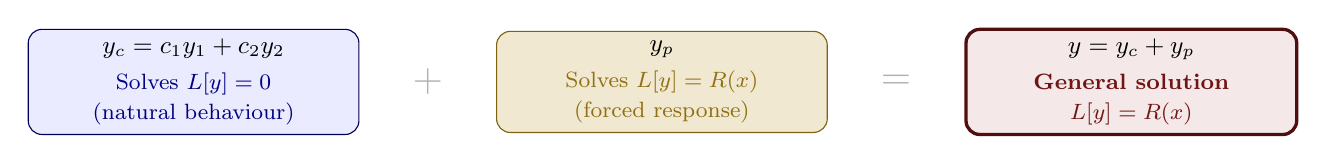
\begin{tikzpicture}[
    node distance=1.6cm,
    box/.style={draw, rounded corners=5pt, minimum width=4.2cm,
                minimum height=0.85cm, align=center, font=\small},
    cbox/.style={box, fill=blue!8, draw=blue!35!black},
    pbox/.style={box, fill=accentgold!20, draw=accentgold!70!black},
    gbox/.style={box, fill=brickred!10, draw=brickred!50!black,
                 very thick, font=\small\bfseries},
    plus/.style={font=\Large\bfseries, color=gray!60},
    arr/.style={->, >=Stealth, thick, gray!60}
  ]
  \node[cbox] (yc) {$y_c = c_1 y_1 + c_2 y_2$\\[2pt]
    {\footnotesize\color{blue!50!black} Solves $L[y]=0$}\\
    {\footnotesize\color{blue!50!black} (natural behaviour)}};
  \node[plus, right=0.55cm of yc] (pl) {$+$};
  \node[pbox, right=0.55cm of pl] (yp) {$y_p$\\[2pt]
    {\footnotesize\color{accentgold!80!black} Solves $L[y]=R(x)$}\\
    {\footnotesize\color{accentgold!80!black} (forced response)}};
  \node[plus, right=0.55cm of yp] (eq) {$=$};
  \node[gbox, right=0.55cm of eq] (y) {$y = y_c + y_p$\\[2pt]
    {\footnotesize\color{brickred!70!black} General solution}\\
    {\footnotesize\color{brickred!70!black} $L[y]=R(x)$}};
\end{tikzpicture}
\caption{The complementary-plus-particular decomposition. Every solution of a
non-homogeneous linear ODE is uniquely expressible as the sum of the
complementary function and a particular solution.}
\label{fig:decomp}
\end{figure}

% ─────────────────────────────────────────────────────────────────────────────
\section{Method I: Undetermined Coefficients}
% ─────────────────────────────────────────────────────────────────────────────

\subsection{The Core Idea}

The method of undetermined coefficients exploits a simple observation: if
$R(x)$ belongs to one of a handful of special families --- polynomials,
exponentials, sines, cosines, and their products --- then $y_p$ belongs to
the \emph{same family}. We therefore \emph{guess} the form of $y_p$ with unknown
coefficients, substitute into the ODE, and solve for those coefficients by
matching both sides.

Why does this work? Because differentiation maps each of these families into
itself: the derivative of a polynomial is a polynomial; the derivative of
$\ee^{\alpha x}$ is $\ee^{\alpha x}$; the derivative of $\sin\beta x$ is
$\cos\beta x$ (which is in the same combined family). The right-hand side can
therefore always be matched.

\begin{procedurebox}{The Trial Function Table}
For the non-homogeneous equation $ay'' + by' + cy = R(x)$, the trial particular
solution $y_p$ is chosen as follows. Let $s$ be the smallest non-negative integer
such that no term in the trial function duplicates a term in the complementary
function $y_c$.

\vspace{6pt}
\renewcommand{\arraystretch}{1.45}
\begin{tabular}{>{\bfseries}p{5.2cm} p{5.8cm}}
\toprule
\rowcolor{midblue!14}
Forcing term $R(x)$ & Trial function $y_p$ \\
\midrule
$P_n(x)$ (polynomial, degree $n$) &
  $x^s(A_n x^n + \cdots + A_1 x + A_0)$ \\
\rowcolor{gray!8}
$\ee^{\alpha x}$ &
  $x^s A\,\ee^{\alpha x}$ \\
$\cos\beta x$ or $\sin\beta x$ &
  $x^s(A\cos\beta x + B\sin\beta x)$ \\
\rowcolor{gray!8}
$P_n(x)\,\ee^{\alpha x}$ &
  $x^s\,(A_n x^n+\cdots+A_0)\ee^{\alpha x}$ \\
$\ee^{\alpha x}\cos\beta x$ or $\ee^{\alpha x}\sin\beta x$ &
  $x^s\,\ee^{\alpha x}(A\cos\beta x + B\sin\beta x)$ \\
\rowcolor{gray!8}
$P_n(x)\,\ee^{\alpha x}\cos\beta x$ &
  $x^s\,\ee^{\alpha x}[(A_n x^n+\cdots)\cos\beta x$\\
or $P_n(x)\,\ee^{\alpha x}\sin\beta x$ &
  $\quad +(B_n x^n+\cdots)\sin\beta x]$ \\
\bottomrule
\end{tabular}
\vspace{4pt}

\textbf{Key rule:} if any part of the natural trial function appears in $y_c$,
multiply the entire trial function by $x^s$ where $s$ is the multiplicity of
the coinciding root. This is the \emph{modification rule}.
\end{procedurebox}

\subsection{The Modification Rule: Resonance}

The most important --- and easily forgotten --- detail is the modification rule.
It arises precisely when the forcing frequency \emph{matches} the natural frequency
of the system: the phenomenon of \textbf{resonance}. In this case, the naive trial
function $y_p$ is already part of $y_c$, so substituting it into the ODE gives
zero on the left, not $R(x)$. The fix is to multiply by $x$ (or $x^2$ for a
repeated root). We will see this explicitly in Example~4.4.

\begin{warningbox}{The Most Common Mistake}
Forgetting to check for resonance is the single most frequent error in this method.
\textbf{Before writing your trial function}, always compare the proposed $y_p$ against
every term in $y_c$. If any term coincides, multiply the trial by $x^s$ (where $s$
is the multiplicity of the problematic root).
\end{warningbox}

% ─────────────────────────────────────────────────────────────────────────────
\section{Worked Examples --- Method of Undetermined Coefficients}
% ─────────────────────────────────────────────────────────────────────────────

\begin{example}{Example 4.1 --- Polynomial Forcing (Foundational)}
Solve $\;y'' - 3y' + 2y = 4x^2$.

\medskip
\textbf{Step 1: Complementary function.}
Characteristic equation: $\lambda^2 - 3\lambda + 2 = (\lambda-1)(\lambda-2)=0$,
roots $\lambda = 1, 2$.
\[
  y_c = c_1\,\ee^{x} + c_2\,\ee^{2x}.
\]

\textbf{Step 2: Trial function.} $R(x) = 4x^2$ is a degree-2 polynomial.
No resonance (neither $\ee^x$ nor $\ee^{2x}$ is a polynomial), so $s=0$:
\[
  y_p = Ax^2 + Bx + C.
\]

\textbf{Step 3: Determine coefficients.}
$y_p' = 2Ax+B$, $\;y_p'' = 2A$. Substituting:
\[
  2A - 3(2Ax+B) + 2(Ax^2+Bx+C) = 4x^2.
\]
Collecting by powers of $x$:
\begin{align*}
  x^2 &: \quad 2A = 4 \implies A = 2,\\
  x^1 &: \quad -6A + 2B = 0 \implies B = 6,\\
  x^0 &: \quad 2A - 3B + 2C = 0 \implies 4 - 18 + 2C = 0 \implies C = 7.
\end{align*}
So $y_p = 2x^2 + 6x + 7$.

\textbf{General solution:}
\[
  \boxed{y = c_1\,\ee^x + c_2\,\ee^{2x} + 2x^2 + 6x + 7.}
\]
\end{example}

% ─────────────────────────────────────────────────────────────────────────────

\begin{example}{Example 4.2 --- Exponential Forcing (Foundational)}
Solve $\;y'' + y' - 6y = 10\,\ee^{3x}$.

\medskip
\textbf{Complementary function.}
Roots: $\lambda^2+\lambda-6=(\lambda+3)(\lambda-2)=0$, so $\lambda=-3,\,2$.
\[
  y_c = c_1\,\ee^{-3x} + c_2\,\ee^{2x}.
\]

\textbf{Trial function.} $R(x) = 10\ee^{3x}$, so try $y_p = A\ee^{3x}$.
Neither $\ee^{-3x}$ nor $\ee^{2x}$ equals $\ee^{3x}$, so no modification needed.

\textbf{Substituting:} $y_p'=3A\ee^{3x}$, $y_p''=9A\ee^{3x}$.
\[
  9A\ee^{3x} + 3A\ee^{3x} - 6A\ee^{3x} = 10\ee^{3x}
  \implies 6A = 10 \implies A = \tfrac{5}{3}.
\]

\textbf{General solution:}
\[
  \boxed{y = c_1\,\ee^{-3x} + c_2\,\ee^{2x} + \tfrac{5}{3}\,\ee^{3x}.}
\]
\end{example}

% ─────────────────────────────────────────────────────────────────────────────

\begin{example}{Example 4.3 --- Sinusoidal Forcing (Foundational)}
Solve $\;y'' + 4y = 3\sin 2x$.

\medskip
\textbf{Complementary function.}
Characteristic equation: $\lambda^2+4=0$, roots $\lambda=\pm 2\ii$.
\[
  y_c = c_1\cos 2x + c_2\sin 2x.
\]

\textbf{Check for resonance.} The natural trial for $\sin 2x$ would be
$y_p = A\cos 2x + B\sin 2x$, but \emph{both} these terms already appear in $y_c$.
This is resonance. Multiply by $x$:
\[
  y_p = x(A\cos 2x + B\sin 2x).
\]

\textbf{Derivatives.}
\begin{align*}
  y_p' &= (A\cos 2x + B\sin 2x) + x(-2A\sin 2x + 2B\cos 2x),\\
  y_p'' &= (-2A\sin 2x + 2B\cos 2x) + (-2A\sin 2x + 2B\cos 2x)
           + x(-4A\cos 2x - 4B\sin 2x)\\
        &= 4B\cos 2x - 4A\sin 2x - 4x(A\cos 2x + B\sin 2x).
\end{align*}

\textbf{Substituting into $y''+4y$:}
\[
  4B\cos 2x - 4A\sin 2x - 4x(\cdots) + 4x(\cdots) = 3\sin 2x.
\]
The $x$-dependent terms cancel exactly (as they must in resonance problems):
\[
  4B\cos 2x - 4A\sin 2x = 3\sin 2x.
\]
Matching coefficients: $4B = 0 \Rightarrow B = 0$ and $-4A = 3 \Rightarrow A = -\tfrac{3}{4}$.

\textbf{General solution:}
\[
  \boxed{y = c_1\cos 2x + c_2\sin 2x - \tfrac{3}{4}\,x\cos 2x.}
\]

The particular solution grows linearly in amplitude with $x$ --- a hallmark of
resonance. This is the mathematical origin of resonance catastrophe in engineering.
\end{example}

% ─────────────────────────────────────────────────────────────────────────────

\begin{example}{Example 4.4 --- Exponential Resonance (Intermediate)}
Solve $\;y'' - 2y' + y = \ee^{x}$, $\quad y(0)=0,\;y'(0)=1$.

\medskip
\textbf{Complementary function.}
$\lambda^2 - 2\lambda + 1 = (\lambda-1)^2 = 0$: repeated root $\lambda=1$.
\[
  y_c = (c_1 + c_2 x)\,\ee^x.
\]

\textbf{Trial function.} The natural trial $A\ee^x$ is already in $y_c$
(multiplicity 2), so we must multiply by $x^2$:
\[
  y_p = Ax^2\ee^x.
\]

\textbf{Derivatives.}
\begin{align*}
  y_p' &= A(2x + x^2)\ee^x,\\
  y_p'' &= A(2 + 4x + x^2)\ee^x.
\end{align*}
Substituting:
\[
  A(2+4x+x^2)\ee^x - 2A(2x+x^2)\ee^x + Ax^2\ee^x = \ee^x.
\]
All $x$- and $x^2$-bearing terms cancel:
\[
  2A\ee^x = \ee^x \implies A = \tfrac{1}{2}.
\]

\textbf{General solution:} $y = (c_1 + c_2 x)\ee^x + \tfrac{1}{2}x^2\ee^x$.

\textbf{Initial conditions:}
$y(0) = c_1 = 0$.
$y'(x) = c_2\ee^x + (c_1+c_2 x)\ee^x + x\ee^x + \tfrac{1}{2}x^2\ee^x$, so
$y'(0) = c_2 + c_1 = c_2 = 1$.

\textbf{Particular (to this IVP) solution:}
\[
  \boxed{y = x\ee^x + \tfrac{1}{2}x^2\ee^x = \tfrac{x}{2}(2+x)\,\ee^x.}
\]
\end{example}

% ─────────────────────────────────────────────────────────────────────────────

\begin{example}{Example 4.5 --- Mixed Forcing: Exponential $\times$ Trig (Intermediate)}
Solve $\;y'' - 2y' + 5y = \ee^x\cos 2x$.

\medskip
\textbf{Complementary function.}
Characteristic roots: $\lambda = \dfrac{2\pm\sqrt{4-20}}{2} = 1 \pm 2\ii$.
\[
  y_c = \ee^x(c_1\cos 2x + c_2\sin 2x).
\]

\textbf{Check resonance.} The natural trial for $\ee^x\cos 2x$ is
$\ee^x(A\cos 2x + B\sin 2x)$. But both terms \emph{appear in $y_c$}. This is
resonance; multiply by $x$:
\[
  y_p = x\,\ee^x(A\cos 2x + B\sin 2x).
\]

\textbf{Derivatives} (product rule, twice):
\begin{align*}
  y_p' &= \ee^x\bigl[(A+Bx\cdot 2 - Ax\cdot 2 + A)\cos 2x
          + (\ldots)\sin 2x\bigr]\\
  &= \ee^x\bigl[(A+2Bx-2Ax+A)\cos 2x + (B-2Ax+2Bx+B)\sin 2x\bigr].
\end{align*}
This is algebraically involved; we proceed systematically. Let
$f = x\cos 2x$ and $g = x\sin 2x$. Then:
\begin{align*}
  \frac{d^2}{dx^2}\bigl[\ee^x f\bigr]
  &= \ee^x(f'' + 2f' + f),\\
  \frac{d^2}{dx^2}\bigl[\ee^x g\bigr]
  &= \ee^x(g'' + 2g' + g).
\end{align*}
Compute: $f'' = -4f + 2(-\sin 2x) \cdot 0 - 4x\cos 2x + \ldots$ --- rather than
expand everything, substitute $y_p$ directly into $y'' - 2y' + 5y$. Using the
operator identity $L[\ee^x u] = \ee^x\bigl[u'' + 2u' + u - 2(u'+u) + 5u\bigr]
= \ee^x[u'' + 4u]$:
\[
  L[y_p] = \ee^x\bigl[(x(A\cos 2x + B\sin 2x))'' + 4x(A\cos 2x+B\sin 2x)\bigr].
\]
Let $h = x(A\cos 2x + B\sin 2x)$. Then:
\begin{align*}
  h' &= (A\cos 2x+B\sin 2x) + x(-2A\sin 2x+2B\cos 2x),\\
  h'' &= 2(-2A\sin 2x+2B\cos 2x) + x(-4A\cos 2x-4B\sin 2x)\\
      &= -4Ax\cos 2x - 4Bx\sin 2x - 4A\sin 2x + 4B\cos 2x.
\end{align*}
So $h'' + 4h = 4B\cos 2x - 4A\sin 2x$ (the $x$-terms cancel). Therefore:
\[
  L[y_p] = \ee^x(4B\cos 2x - 4A\sin 2x) = \ee^x\cos 2x.
\]
Matching: $4B = 1$, $-4A = 0$, giving $A = 0$, $B = \tfrac{1}{4}$.

\textbf{General solution:}
\[
  \boxed{y = \ee^x\!\left(c_1\cos 2x + c_2\sin 2x + \tfrac{x}{4}\sin 2x\right).}
\]
The linearly growing amplitude $\frac{x}{4}$ in the particular solution once again
signals resonance: the forcing frequency $2$ exactly matches the imaginary part of
the characteristic roots.
\end{example}

% ─────────────────────────────────────────────────────────────────────────────

\begin{example}{Example 4.6 --- Superposition of Forcing Terms (Intermediate)}
Solve $\;y'' + y = 2\sin x + x^2 - 1$.

\medskip
\textbf{Complementary function.} $\lambda^2+1=0 \Rightarrow \lambda=\pm\ii$.
\[
  y_c = c_1\cos x + c_2\sin x.
\]

By the \textbf{superposition principle for the right-hand side}, we handle each
forcing term separately.

\textbf{Part A:} $R_1 = 2\sin x$. Trial: $A\cos x + B\sin x$ --- both in $y_c$.
Resonance. Multiply by $x$:
\[
  y_{p1} = x(A\cos x + B\sin x).
\]
Substituting (same computation as Example~4.3 pattern):
$2B\cos x - 2A\sin x = 2\sin x \Rightarrow B=0,\; A=-1$.
\[
  y_{p1} = -x\cos x.
\]

\textbf{Part B:} $R_2 = x^2 - 1$. Trial: $Cx^2+Dx+E$. No resonance.
\[
  (2C) + (Cx^2+Dx+E) = x^2-1.
\]
Matching: $C=1$, $D=0$, $2C+E=-1 \Rightarrow E=-3$.
\[
  y_{p2} = x^2 - 3.
\]

\textbf{General solution:}
\[
  \boxed{y = c_1\cos x + c_2\sin x - x\cos x + x^2 - 3.}
\]
\end{example}

% ─────────────────────────────────────────────────────────────────────────────
\section{Method II: Variation of Parameters}
% ─────────────────────────────────────────────────────────────────────────────

\subsection{Motivation and Derivation}

The method of undetermined coefficients fails when $R(x)$ is not of the
``nice'' exponential-polynomial-trig form. For example, $R(x) = \tan x$,
$R(x) = 1/x$, or $R(x) = \ln x$ cannot be handled by guessing. We need a
method that works for \emph{any} continuous $R(x)$.

\textbf{The key idea}: instead of fixing the constants $c_1, c_2$ in the
complementary function, allow them to be \emph{functions of $x$}. Write
\[
  y_p = u_1(x)\,y_1(x) + u_2(x)\,y_2(x),
\]
where $y_1, y_2$ is the known fundamental set, and $u_1, u_2$ are to be
determined. The ``varying'' of the parameters $c_1 \to u_1(x)$,
$c_2 \to u_2(x)$ is why the method is called variation of parameters.

We have two unknowns ($u_1', u_2'$) and one equation (the ODE). The extra
degree of freedom is used to impose the \textbf{simplifying condition}:
\[
  u_1'(x)\,y_1(x) + u_2'(x)\,y_2(x) = 0.
\]
This keeps $y_p'$ clean (no second derivatives of $u_1, u_2$ in $y_p'$) and
leads to a Cramer's rule system.

\begin{theorembox}{Theorem 5.1 --- Variation of Parameters Formula}
Let $y_1, y_2$ be a fundamental set for $y'' + P(x)y' + Q(x)y = 0$, with Wronskian
$W = W(y_1,y_2) \neq 0$. A particular solution of $y'' + P(x)y' + Q(x)y = R(x)$
is
\[
  y_p = -y_1(x)\int\frac{y_2(x)\,R(x)}{W(x)}\,\dd x
        + y_2(x)\int\frac{y_1(x)\,R(x)}{W(x)}\,\dd x.
\]
Equivalently, solve the $2\times 2$ system
\[
  \begin{pmatrix}y_1 & y_2\\y_1' & y_2'\end{pmatrix}
  \begin{pmatrix}u_1'\\u_2'\end{pmatrix}
  =
  \begin{pmatrix}0\\R(x)\end{pmatrix}
\]
by Cramer's rule:
\[
  u_1' = \frac{-y_2 R}{W}, \qquad u_2' = \frac{y_1 R}{W}.
\]
Then $u_1 = \int u_1'\,\dd x$ and $u_2 = \int u_2'\,\dd x$ (no constants of
integration needed; they merge into $y_c$).
\end{theorembox}

\textit{Derivation outline.} Impose $u_1'y_1 + u_2'y_2 = 0$. Then
$y_p' = u_1 y_1' + u_2 y_2'$. Differentiating again and substituting into
$y_p'' + Py_p' + Qy_p = R$ uses $L[y_1] = L[y_2] = 0$ to eliminate
$u_1, u_2$, leaving $u_1'y_1' + u_2'y_2' = R$. Together with the simplifying
condition, this gives the $2\times 2$ system above. $\square$

\begin{figure}[H]
\centering
\begin{tikzpicture}[
    node distance=1.2cm,
    step/.style={draw, rounded corners=5pt, minimum width=8cm,
                 minimum height=0.78cm, align=center, font=\small,
                 fill=blue!5, draw=blue!30!black},
    arr/.style={->, >=Stealth, thick, midblue!60}
  ]
  \node[step] (s1) {\textbf{1.} Find $y_1, y_2$ from $y'' + Py' + Qy = 0$ and compute $W$};
  \node[step, below=of s1] (s2)
    {\textbf{2.} Compute $u_1' = -y_2 R / W$ and $u_2' = y_1 R / W$};
  \node[step, below=of s2] (s3)
    {\textbf{3.} Integrate: $u_1 = \int u_1'\,\dd x$, $\;u_2 = \int u_2'\,\dd x$};
  \node[step, below=of s3] (s4)
    {\textbf{4.} Particular solution: $y_p = u_1 y_1 + u_2 y_2$};
  \node[step, below=of s4, fill=brickred!8, draw=brickred!40!black] (s5)
    {\textbf{5.} General solution: $y = c_1 y_1 + c_2 y_2 + y_p$};
  \draw[arr] (s1)--(s2); \draw[arr] (s2)--(s3);
  \draw[arr] (s3)--(s4); \draw[arr] (s4)--(s5);
\end{tikzpicture}
\caption{Step-by-step flowchart for the method of variation of parameters.}
\label{fig:vop}
\end{figure}

% ─────────────────────────────────────────────────────────────────────────────
\section{Worked Examples --- Variation of Parameters}
% ─────────────────────────────────────────────────────────────────────────────

\begin{example}{Example 6.1 --- Tangent Forcing (Foundational)}
Solve $\;y'' + y = \tan x$.

\medskip
\textbf{Complementary function.} $\lambda^2+1=0 \Rightarrow \lambda=\pm\ii$.
\[
  y_1 = \cos x, \quad y_2 = \sin x, \qquad
  W = \cos x\cdot\cos x - \sin x\cdot(-\sin x) = 1.
\]

\textbf{Applying the formula} ($R = \tan x$, $W = 1$):
\[
  u_1' = -\frac{y_2 R}{W} = -\sin x\tan x = -\frac{\sin^2 x}{\cos x}
       = \cos x - \sec x,
\]
\[
  u_2' = \frac{y_1 R}{W} = \cos x\tan x = \sin x.
\]

\textbf{Integrating:}
\[
  u_1 = \sin x - \ln|\sec x + \tan x|,
\]
\[
  u_2 = -\cos x.
\]

\textbf{Particular solution:}
\begin{align*}
  y_p &= u_1\cos x + u_2\sin x\\
      &= (\sin x - \ln|\sec x+\tan x|)\cos x + (-\cos x)\sin x\\
      &= -\cos x\,\ln|\sec x + \tan x|.
\end{align*}

\textbf{General solution:}
\[
  \boxed{y = c_1\cos x + c_2\sin x - \cos x\,\ln|\sec x + \tan x|.}
\]
This is a valid particular solution on any interval where $\sec x + \tan x > 0$,
for example $(-\pi/2,\,\pi/2)$.
\end{example}

% ─────────────────────────────────────────────────────────────────────────────

\begin{example}{Example 6.2 --- Reciprocal Forcing (Foundational)}
Solve $\;y'' - 3y' + 2y = \dfrac{\ee^x}{1+\ee^x}$.

\medskip
\textbf{Complementary function.}
$\lambda^2-3\lambda+2=(\lambda-1)(\lambda-2)=0$, $\lambda=1,2$.
\[
  y_1 = \ee^x,\quad y_2 = \ee^{2x},\qquad
  W = 2\ee^{3x} - \ee^{3x} = \ee^{3x}.
\]

\textbf{Variation formulas} ($R = \ee^x/(1+\ee^x)$):
\[
  u_1' = \frac{-\ee^{2x}\cdot\dfrac{\ee^x}{1+\ee^x}}{\ee^{3x}}
       = \frac{-1}{1+\ee^x},
\]
\[
  u_2' = \frac{\ee^x\cdot\dfrac{\ee^x}{1+\ee^x}}{\ee^{3x}}
       = \frac{\ee^{-x}}{1+\ee^x} = \ee^{-x} - \frac{\ee^{-x}}{1+\ee^x}
       = \ee^{-x} - \frac{1}{\ee^x(1+\ee^x)}.
\]
A neater approach: write $u_2' = \ee^{-2x}\cdot\dfrac{\ee^x}{1+\ee^x}
= \dfrac{\ee^{-x}}{1+\ee^x}$.

\textbf{Integrating:}
\[
  u_1 = -\int\frac{dx}{1+\ee^x}.
\]
Let $t=\ee^x$: $u_1 = -\int\dfrac{dt}{t(1+t)} = -\int\!\left(\dfrac{1}{t}-\dfrac{1}{1+t}\right)dt
= -x + \ln(1+\ee^x)$.

\[
  u_2 = \int\frac{\ee^{-x}}{1+\ee^x}\,dx.
\]
Let $t=\ee^x$: $u_2 = \int\dfrac{t^{-1}}{1+t}\cdot\dfrac{dt}{t}
= \int\dfrac{dt}{t^2(1+t)}$, which gives
$u_2 = \dfrac{1}{\ee^x} + \ln\ee^x - \ln(1+\ee^x) + \text{const}
= \ee^{-x} + \ln\!\left(\dfrac{\ee^x}{1+\ee^x}\right)$.

\textbf{Particular solution}:
\[
  y_p = \ee^x\!\left(-x + \ln(1+\ee^x)\right)
        + \ee^{2x}\!\left(\ee^{-x} + \ln\tfrac{\ee^x}{1+\ee^x}\right).
\]
Simplifying:
\[
  y_p = -x\ee^x + \ee^x\ln(1+\ee^x) + \ee^x + \ee^{2x}\ln\ee^x
        - \ee^{2x}\ln(1+\ee^x).
\]
The $\ee^x$ term merges into $c_1\ee^x$, and the $x$-terms remain:
\[
  \boxed{y = c_1\ee^x + c_2\ee^{2x} - x\ee^x
          + (\ee^x-\ee^{2x})\ln(1+\ee^x).}
\]
\end{example}

% ─────────────────────────────────────────────────────────────────────────────

\begin{example}{Example 6.3 --- Logarithmic Forcing (Intermediate)}
Solve $\;x^2 y'' - 2xy' + 2y = x^2\ln x, \quad x > 0$.

\medskip
This is an \textbf{Euler--Cauchy} equation. The substitution $y=x^\lambda$ gives
the characteristic equation $\lambda(\lambda-1)-2\lambda+2=0$, i.e.\ $\lambda^2-3\lambda+2=0$,
roots $\lambda=1,2$.
\[
  y_c = c_1 x + c_2 x^2.
\]

\textbf{Writing in standard form}: divide by $x^2$:
\[
  y'' - \frac{2}{x}\,y' + \frac{2}{x^2}\,y = \ln x.
\]
So $P(x) = -2/x$, $Q(x)=2/x^2$, $R(x)=\ln x$.

\textbf{Wronskian:}
\[
  W(x,x^2) = x\cdot 2x - x^2\cdot 1 = x^2.
\]

\textbf{Variation:}
\[
  u_1' = \frac{-x^2\ln x}{x^2} = -\ln x, \qquad
  u_2' = \frac{x\ln x}{x^2} = \frac{\ln x}{x}.
\]

\textbf{Integrating} (by parts):
\[
  u_1 = -\int \ln x\,dx = -(x\ln x - x) = x - x\ln x,
\]
\[
  u_2 = \int\frac{\ln x}{x}\,dx = \frac{(\ln x)^2}{2}.
\]

\textbf{Particular solution:}
\[
  y_p = (x - x\ln x)\cdot x + \frac{(\ln x)^2}{2}\cdot x^2
      = x^2 - x^2\ln x + \frac{x^2(\ln x)^2}{2}.
\]
The $x^2$ term merges into $c_2 x^2$:
\[
  \boxed{y = c_1 x + c_2 x^2 + x^2\!\left[\frac{(\ln x)^2}{2} - \ln x\right].}
\]
\end{example}

% ─────────────────────────────────────────────────────────────────────────────

\begin{example}{Example 6.4 --- Secant Forcing, IVP (Intermediate)}
Solve $\;y'' + 4y = 8\sec^2 2x$, $\quad y(0) = 1$, $\;y'(0) = 0$.

\medskip
\textbf{Complementary function.} $\lambda^2+4=0 \Rightarrow \lambda=\pm 2\ii$.
\[
  y_1 = \cos 2x,\quad y_2=\sin 2x,\quad W=2.
\]

\textbf{Variation:}
\[
  u_1' = \frac{-\sin 2x\cdot 8\sec^2 2x}{2} = -4\frac{\sin 2x}{\cos^2 2x}
       = -4\sec 2x\tan 2x,
\]
\[
  u_2' = \frac{\cos 2x\cdot 8\sec^2 2x}{2} = 4\sec 2x.
\]

\textbf{Integrating:}
\[
  u_1 = -4\int\sec 2x\tan 2x\,dx = -4\cdot\tfrac{1}{2}\sec 2x = -2\sec 2x,
\]
\[
  u_2 = 4\int\sec 2x\,dx = 4\cdot\tfrac{1}{2}\ln|\sec 2x + \tan 2x|
       = 2\ln|\sec 2x + \tan 2x|.
\]

\textbf{Particular solution:}
\[
  y_p = -2\sec 2x\cdot\cos 2x + 2\sin 2x\ln|\sec 2x+\tan 2x|
      = -2 + 2\sin 2x\ln|\sec 2x+\tan 2x|.
\]

\textbf{General solution:}
\[
  y = c_1\cos 2x + c_2\sin 2x - 2 + 2\sin 2x\ln|\sec 2x+\tan 2x|.
\]

\textbf{Initial conditions:} $y(0) = c_1 - 2 = 1 \Rightarrow c_1 = 3$.
$y'(0) = -2c_1\sin 0 + 2c_2\cos 0 + (\text{terms})|_{x=0} = 2c_2 = 0 \Rightarrow c_2=0$.

\[
  \boxed{y = 3\cos 2x - 2 + 2\sin 2x\ln|\sec 2x+\tan 2x|.}
\]
\end{example}

% ─────────────────────────────────────────────────────────────────────────────
\section{Applications in Physics}
% ─────────────────────────────────────────────────────────────────────────────

The non-homogeneous equation is the equation of \emph{driven} systems. The homogeneous
Part~2 described what a system does in isolation; now we describe what happens when
you push it. The richness of the response --- including resonance, beats, and transient
vs.\ steady-state behaviour --- all flow from the structure of Theorem~2.1.

\subsection{The Driven Harmonic Oscillator}

Add a periodic external force $F_0\cos\omega t$ to the undamped spring equation:
\begin{equation}
  \ddot{x} + \omega_0^2 x = \frac{F_0}{m}\cos\omega t.
  \label{eq:driven}
\end{equation}
This is the archetype of all driven oscillator problems.

\subsubsection*{Case A: Off-resonance ($\omega \neq \omega_0$)}

The complementary function is $x_c = c_1\cos\omega_0 t + c_2\sin\omega_0 t$.
The trial $x_p = A\cos\omega t + B\sin\omega t$ does not clash with $x_c$
($\omega \neq \omega_0$), so no modification is needed.
Substituting: $-A\omega^2\cos\omega t + A\omega_0^2\cos\omega t = \frac{F_0}{m}\cos\omega t$,
giving $B = 0$ and
\[
  A = \frac{F_0/m}{\omega_0^2 - \omega^2}.
\]

\textbf{General solution:}
\[
  x(t) = c_1\cos\omega_0 t + c_2\sin\omega_0 t
          + \frac{F_0/m}{\omega_0^2-\omega^2}\cos\omega t.
\]
With $x(0)=0$, $\dot x(0)=0$: $c_1 = -F_0/(m(\omega_0^2-\omega^2))$, $c_2=0$:
\begin{equation}
  \boxed{x(t) = \frac{F_0/m}{\omega_0^2-\omega^2}(\cos\omega t - \cos\omega_0 t).}
  \label{eq:beats}
\end{equation}

Using the identity $\cos A - \cos B = -2\sin\!\tfrac{A+B}{2}\sin\!\tfrac{A-B}{2}$,
for $\omega$ close to $\omega_0$ this becomes approximately a
\emph{slowly amplitude-modulated} oscillation: the phenomenon of \textbf{beats}.

\subsubsection*{Case B: Resonance ($\omega = \omega_0$)}

The trial $A\cos\omega_0 t$ is already in $x_c$. Multiply by $t$:
$x_p = t(A\cos\omega_0 t + B\sin\omega_0 t)$.
Substituting (see Example~4.3 pattern):
\[
  A = 0, \qquad B = \frac{F_0}{2m\omega_0}.
\]
\[
  \boxed{x_p = \frac{F_0}{2m\omega_0}\,t\sin\omega_0 t.}
\]
The amplitude grows \emph{without bound} as $t\to\infty$ --- pure resonance.
This is the Tacoma Narrows bridge disaster in mathematical form.

\begin{figure}[H]
\centering
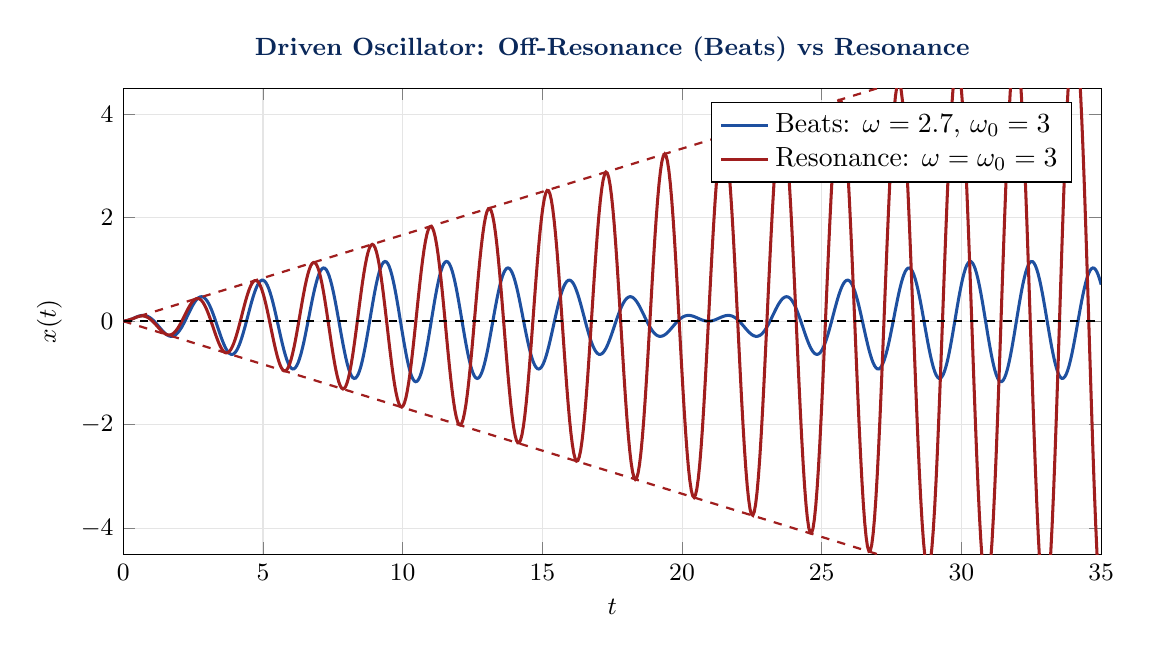
\begin{tikzpicture}
\begin{axis}[
  width=14cm, height=7.5cm,
  xlabel={$t$}, ylabel={$x(t)$},
  title={\textbf{Driven Oscillator: Off-Resonance (Beats) vs Resonance}},
  xmin=0, xmax=35,
  ymin=-4.5, ymax=4.5,
  legend pos=north east,
  legend cell align={left},
  grid=both, grid style={gray!20},
  tick label style={font=\small},
  label style={font=\small},
  title style={font=\small\bfseries, color=deepblue},
  every axis plot/.append style={line width=1.1pt},
]
% Off-resonance beats: omega0=3, omega=2.7, F0/m=1
% x = 1/(9-7.29)*(cos(2.7t)-cos(3t)) = (1/1.71)*(cos(2.7t)-cos(3t))
\addplot[color=midblue, domain=0:35, samples=700]
  {(1/1.71)*(cos(deg(2.7*x)) - cos(deg(3*x)))};
\addlegendentry{Beats: $\omega=2.7$, $\omega_0=3$}

% Resonance: omega=omega0=3, x_p = t*sin(3t)/(2*3) = t*sin(3t)/6
\addplot[color=brickred, domain=0:35, samples=700]
  {x*sin(deg(3*x))/6};
\addlegendentry{Resonance: $\omega=\omega_0=3$}

% Resonance envelope
\addplot[brickred, dashed, line width=0.8pt, domain=0:35, samples=100]
  {x/6};
\addplot[brickred, dashed, line width=0.8pt, domain=0:35, samples=100]
  {-x/6};

\addplot[black, dashed, line width=0.5pt] coordinates {(0,0)(35,0)};
\end{axis}
\end{tikzpicture}
\caption{Two solutions of $\ddot x + 9x = \cos\omega t$ with $x(0)=0$,
$\dot x(0)=0$. Blue: off-resonance ($\omega=2.7$), producing beats --- a slow
amplitude modulation. Red: resonance ($\omega=\omega_0=3$), producing linearly
growing amplitude (dashed red lines are the $\pm t/(2\omega_0)$ envelope). The
resonance solution eventually dominates all practical systems.}
\label{fig:resonance}
\end{figure}

\subsection{The Damped Driven Oscillator: Steady State and Transient}

Add damping ($\zeta > 0$) to the driven equation:
\begin{equation}
  \ddot{x} + 2\zeta\omega_0\dot{x} + \omega_0^2 x = \frac{F_0}{m}\cos\omega t.
  \label{eq:ddo}
\end{equation}
The complementary solution $x_c$ decays to zero (for $\zeta > 0$). The
particular solution
\[
  x_p = C\cos(\omega t - \delta)
\]
persists indefinitely. We call $x_c$ the \textbf{transient} and $x_p$ the
\textbf{steady-state response}.

\begin{theorembox}{Theorem 7.1 --- Steady-State Amplitude and Phase}
For equation \eqref{eq:ddo}, the steady-state amplitude and phase are
\[
  C = \frac{F_0/m}{\sqrt{(\omega_0^2-\omega^2)^2 + (2\zeta\omega_0\omega)^2}},
  \qquad
  \tan\delta = \frac{2\zeta\omega_0\omega}{\omega_0^2 - \omega^2}.
\]
The ratio $C/(F_0/m\omega_0^2)$ is called the \textbf{amplitude response} (or
\textbf{dynamic magnification factor}). It peaks at the \textbf{resonant frequency}
\[
  \omega_r = \omega_0\sqrt{1 - 2\zeta^2} \quad (\text{for } \zeta < 1/\sqrt{2}),
\]
where the peak amplitude is $F_0/(2m\omega_0^2\zeta\sqrt{1-\zeta^2})$.
\end{theorembox}

\begin{figure}[H]
\centering
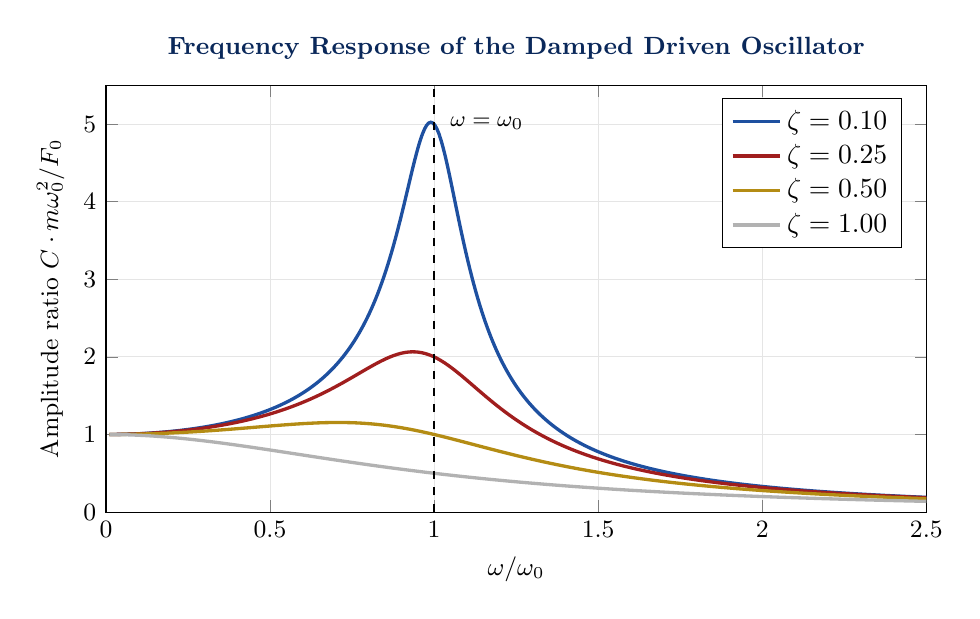
\begin{tikzpicture}
\begin{axis}[
  width=12cm, height=7cm,
  xlabel={$\omega/\omega_0$},
  ylabel={Amplitude ratio $C\cdot m\omega_0^2/F_0$},
  title={\textbf{Frequency Response of the Damped Driven Oscillator}},
  xmin=0, xmax=2.5,
  ymin=0, ymax=5.5,
  legend pos=north east,
  legend cell align={left},
  grid=both, grid style={gray!20},
  tick label style={font=\small},
  label style={font=\small},
  title style={font=\small\bfseries, color=deepblue},
  every axis plot/.append style={line width=1.2pt},
  xtick={0,0.5,1.0,1.5,2.0,2.5},
]
% C = 1/sqrt((1-r^2)^2+(2*zeta*r)^2) where r=omega/omega0
\addplot[color=midblue, domain=0.01:2.5, samples=400]
  {1/sqrt((1-x^2)^2 + (2*0.1*x)^2)};
\addlegendentry{$\zeta = 0.10$}

\addplot[color=brickred, domain=0.01:2.5, samples=400]
  {1/sqrt((1-x^2)^2 + (2*0.25*x)^2)};
\addlegendentry{$\zeta = 0.25$}

\addplot[color=accentgold, domain=0.01:2.5, samples=400]
  {1/sqrt((1-x^2)^2 + (2*0.5*x)^2)};
\addlegendentry{$\zeta = 0.50$}

\addplot[color=gray!60, domain=0.01:2.5, samples=400]
  {1/sqrt((1-x^2)^2 + (2*1.0*x)^2)};
\addlegendentry{$\zeta = 1.00$}

% Mark omega/omega0 = 1
\addplot[black, dashed, line width=0.6pt] coordinates {(1,0)(1,5.5)};
\node[font=\footnotesize, anchor=south west] at (axis cs:1.02,4.8)
  {$\omega=\omega_0$};
\end{axis}
\end{tikzpicture}
\caption{Frequency response curves (Bode-like plots) for the damped driven oscillator.
The peak amplitude occurs slightly below $\omega_0$ for light damping and disappears
for $\zeta \geq 1/\sqrt{2} \approx 0.707$. As $\zeta \to 0$, the resonance peak
diverges, recovering the unbounded resonance of the undamped case.}
\label{fig:freqresp}
\end{figure}

\begin{example}{Example 7.1 --- Driven Damped Oscillator, Full IVP (Intermediate)}
Solve $\;\ddot{x} + 4\dot{x} + 5x = 10\cos 2t$, $\quad x(0)=0$, $\;\dot{x}(0)=0$.

\medskip
\textbf{Complementary function.} Characteristic roots:
$\lambda = \dfrac{-4\pm\sqrt{16-20}}{2} = -2\pm\ii$.
\[
  x_c = \ee^{-2t}(c_1\cos t + c_2\sin t).
\]

\textbf{Particular (steady-state) solution.} Try $x_p = A\cos 2t + B\sin 2t$.
$\ddot x_p = -4A\cos 2t - 4B\sin 2t$, $\;\dot x_p = -2A\sin 2t + 2B\cos 2t$.

Substituting into the ODE:
\begin{align*}
  (-4A+8B+5A)\cos 2t + (-4B-8A+5B)\sin 2t &= 10\cos 2t\\
  (A + 8B)\cos 2t + (B - 8A)\sin 2t &= 10\cos 2t.
\end{align*}
System: $A + 8B = 10$ and $B - 8A = 0 \Rightarrow B = 8A$.
Substituting: $A + 64A = 10 \Rightarrow A = \frac{10}{65} = \frac{2}{13}$,
$B = \frac{16}{13}$.
\[
  x_p = \frac{2}{13}\cos 2t + \frac{16}{13}\sin 2t.
\]

\textbf{General solution:} $x = \ee^{-2t}(c_1\cos t + c_2\sin t) + x_p$.

\textbf{Initial conditions:} $x(0)=0 \Rightarrow c_1 + \tfrac{2}{13} = 0
\Rightarrow c_1 = -\tfrac{2}{13}$.

$\dot x(0)=0$: $\dot x = \ee^{-2t}\bigl[(-2c_1+c_2)\cos t + (-c_1-2c_2)\sin t\bigr]
+ \dot x_p$, so $-2c_1+c_2 + \dot x_p(0) = 0$ where
$\dot x_p(0) = \tfrac{32}{13}$.

$\Rightarrow c_2 = 2c_1 - \tfrac{32}{13} = -\tfrac{4}{13} - \tfrac{32}{13}
= -\tfrac{36}{13}$.

\textbf{Solution:}
\[
  \boxed{x(t) = \ee^{-2t}\!\left(-\tfrac{2}{13}\cos t - \tfrac{36}{13}\sin t\right)
          + \tfrac{2}{13}\cos 2t + \tfrac{16}{13}\sin 2t.}
\]
The first part is the \textbf{transient} (decays to zero); the second is the
\textbf{steady-state} response. After a few time constants $1/2$, only the
steady-state survives.
\end{example}

% ─────────────────────────────────────────────────────────────────────────────
\subsection{Forced RLC Circuits}

Kirchhoff's voltage law for an $RLC$ series circuit driven by a voltage source
$\mathcal{V}(t)$ gives
\begin{equation}
  L\ddot{q} + R\dot{q} + \frac{q}{C} = \mathcal{V}(t),
  \label{eq:rlc_forced}
\end{equation}
where $q(t)$ is the charge on the capacitor. This is \emph{mathematically
identical} to \eqref{eq:ddo} with the correspondences $m\leftrightarrow L$,
$\gamma\leftrightarrow R$, $k\leftrightarrow 1/C$, and $F(t)\leftrightarrow\mathcal{V}(t)$.
Every result from the mechanical oscillator carries over directly.

The table below collects the mechanical-electrical analogy:

\begin{center}
\renewcommand{\arraystretch}{1.3}
\begin{tabular}{lll}
\toprule
\rowcolor{midblue!14}
\textbf{Mechanical} & \textbf{Electrical} & \textbf{Symbol} \\
\midrule
\rowcolor{gray!6}
Mass & Inductance & $m \leftrightarrow L$ \\
Damping coefficient & Resistance & $\gamma \leftrightarrow R$ \\
\rowcolor{gray!6}
Spring constant & Inverse capacitance & $k \leftrightarrow 1/C$ \\
Displacement & Charge & $x \leftrightarrow q$ \\
\rowcolor{gray!6}
Velocity & Current & $\dot x \leftrightarrow I = \dot q$ \\
External force & EMF (voltage) & $F(t) \leftrightarrow \mathcal{V}(t)$ \\
\bottomrule
\end{tabular}
\end{center}

\begin{example}{Example 7.2 --- Forced RLC Circuit (Intermediate)}
An $RLC$ series circuit has $L=1\,\mathrm{H}$, $R=2\,\Omega$, $C=\tfrac{1}{5}\,\mathrm{F}$,
driven by $\mathcal{V}(t) = 5\sin t$ V. Initially $q(0)=0$, $I(0)=\dot q(0)=0$.

\medskip
The ODE is $\ddot q + 2\dot q + 5q = 5\sin t$.

\textbf{Complementary function.} Roots: $\lambda = -1\pm 2\ii$, so
$q_c = \ee^{-t}(c_1\cos 2t + c_2\sin 2t)$.

\textbf{Particular solution.} Try $q_p = A\cos t + B\sin t$:
\[
  (-A + 2B + 5A)\cos t + (-B - 2A + 5B)\sin t = 5\sin t.
\]
$4A + 2B = 0$ and $-2A + 4B = 5$. Solving: $A = -\tfrac{1}{2}$,
$B = 1$.
\[
  q_p = -\tfrac{1}{2}\cos t + \sin t.
\]

\textbf{Initial conditions:} $q(0) = c_1 - \tfrac{1}{2} = 0 \Rightarrow c_1 = \tfrac{1}{2}$.
$\dot q(0) = (-c_1 + 2c_2) + \dot q_p(0) = -\tfrac{1}{2} + 2c_2 + 1 = 0
\Rightarrow c_2 = -\tfrac{1}{4}$.

\textbf{Solution:}
\[
  \boxed{q(t) = \ee^{-t}\!\left(\tfrac{1}{2}\cos 2t - \tfrac{1}{4}\sin 2t\right)
                - \tfrac{1}{2}\cos t + \sin t\;\;\mathrm{C}.}
\]
The current $I = \dot q$ can be found by differentiation. The transient
$\ee^{-t}(\cdots)$ fades after a few seconds; the AC steady-state
$-\tfrac{1}{2}\cos t + \sin t$ remains.
\end{example}

\begin{figure}[H]
\centering
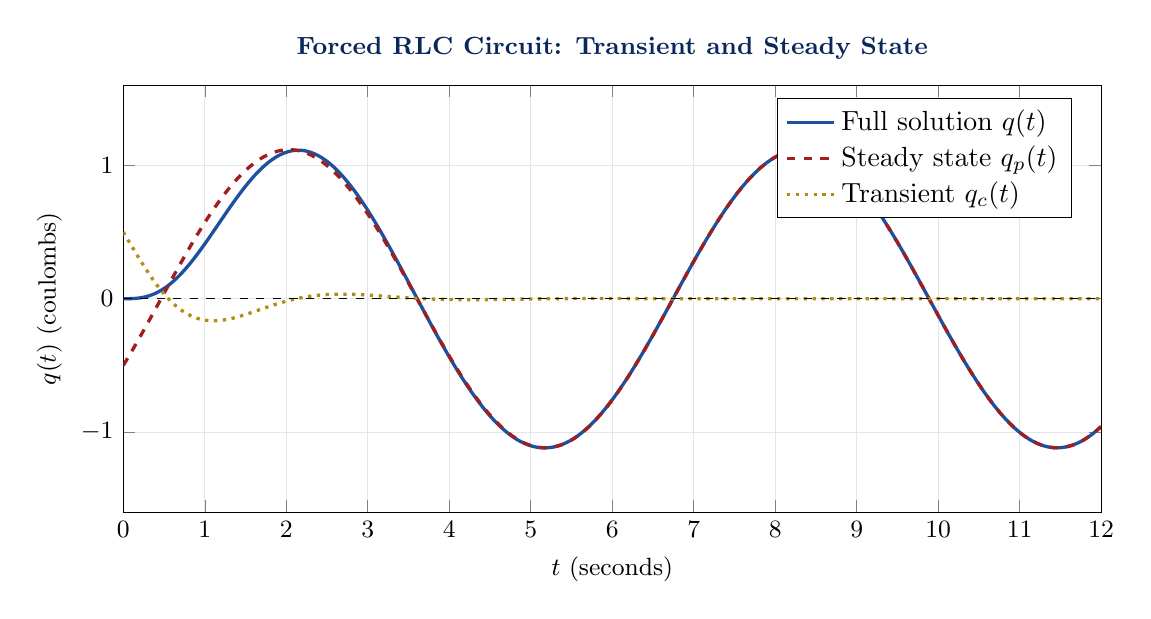
\begin{tikzpicture}
\begin{axis}[
  width=14cm, height=7cm,
  xlabel={$t$ (seconds)},
  ylabel={$q(t)$ (coulombs)},
  title={\textbf{Forced RLC Circuit: Transient and Steady State}},
  xmin=0, xmax=12,
  ymin=-1.6, ymax=1.6,
  legend pos=north east,
  legend cell align={left},
  grid=both, grid style={gray!20},
  tick label style={font=\small},
  label style={font=\small},
  title style={font=\small\bfseries, color=deepblue},
  every axis plot/.append style={line width=1.2pt},
]
% Full solution
\addplot[color=midblue, domain=0:12, samples=500]
  { exp(-x)*(0.5*cos(deg(2*x)) - 0.25*sin(deg(2*x)))
    - 0.5*cos(deg(x)) + sin(deg(x)) };
\addlegendentry{Full solution $q(t)$}

% Steady state only
\addplot[color=brickred, dashed, domain=0:12, samples=300]
  {-0.5*cos(deg(x)) + sin(deg(x))};
\addlegendentry{Steady state $q_p(t)$}

% Transient only
\addplot[color=accentgold, dotted, domain=0:12, samples=300]
  {exp(-x)*(0.5*cos(deg(2*x)) - 0.25*sin(deg(2*x)))};
\addlegendentry{Transient $q_c(t)$}

\addplot[black, dashed, line width=0.5pt] coordinates {(0,0)(12,0)};
\end{axis}
\end{tikzpicture}
\caption{Charge $q(t)$ in the forced RLC circuit of Example~7.2. The full
solution (blue) starts at zero and is initially dominated by the transient
(gold, dotted). After $t\approx 4$--5 seconds, the transient has decayed and
only the sinusoidal steady state (red, dashed) remains.}
\label{fig:rlc_forced}
\end{figure}

% ─────────────────────────────────────────────────────────────────────────────
\subsection{Green's Function: Impulse Response}

Variation of parameters has a deep interpretation. Consider the equation
\[
  y'' + P(x)y' + Q(x)y = R(x).
\]
We can write the particular solution as
\[
  y_p(x) = \int_{x_0}^{x} G(x,\xi)\,R(\xi)\,\dd\xi,
\]
where the \textbf{Green's function}
\[
  G(x,\xi) = \frac{y_1(\xi)\,y_2(x) - y_2(\xi)\,y_1(x)}{W(\xi)}
\]
represents the response at position $x$ to a unit impulse applied at position
$\xi$. This is precisely the variation of parameters formula written as a
convolution. The Green's function is one of the most powerful tools in
mathematical physics: it converts the problem of solving a differential equation
into a problem of integration. Every result we compute by variation of
parameters is secretly a Green's function calculation.

% ─────────────────────────────────────────────────────────────────────────────
\section{Further Remarks}
% ─────────────────────────────────────────────────────────────────────────────

\subsection{When to Use Which Method}

A natural question is: given a non-homogeneous ODE, which method should you reach
for first?

\begin{procedurebox}{Method Selection Guide}
\begin{enumerate}[itemsep=4pt]
  \item \textbf{Is $R(x)$ a polynomial, exponential, sine, cosine, or product of
        these?} $\to$ Try \textbf{undetermined coefficients} first. Check for resonance.
  \item \textbf{Is $R(x)$ something else} (e.g.\ $\tan x$, $\sec x$, $\ln x$,
        $1/(1+x^2)$, a function you cannot differentiate repeatedly and get the same
        form back)? $\to$ Use \textbf{variation of parameters}.
  \item \textbf{Do you need a completely general formula} valid for any $R(x)$?
        $\to$ Use \textbf{variation of parameters} (it always works).
  \item \textbf{Is the equation Euler--Cauchy} ($x^n y^{(n)} + \cdots$)?
        $\to$ First reduce to constant-coefficient form via $x = \ee^t$ (or use
        $y = x^\lambda$ for the homogeneous part), then apply either method to the
        non-homogeneous version.
\end{enumerate}
\end{procedurebox}

\subsection{Superposition for Multiple Forcing Terms}

When $R(x) = R_1(x) + R_2(x) + \cdots + R_k(x)$, the superposition principle
for the \emph{right-hand side} applies: find a particular solution $y_{p_i}$
for each $R_i$ individually, then $y_p = y_{p_1} + \cdots + y_{p_k}$. This is
valid because the operator $L$ is linear. We used this in Example~4.6. The
same principle underlies Fourier analysis: a forcing function is decomposed into
sinusoidal modes, each producing its own particular solution, and the total
response is their sum.

\subsection{Energy Interpretation}

In the driven oscillator $\ddot x + 2\zeta\omega_0\dot x + \omega_0^2 x = (F_0/m)\cos\omega t$,
the instantaneous power delivered by the driving force is $P = F\dot x$. At steady
state ($x_p = C\cos(\omega t - \delta)$), the time-averaged power is
\[
  \langle P\rangle = \frac{F_0^2}{2m}\cdot\frac{2\zeta\omega_0\omega}{(\omega_0^2-\omega^2)^2+(2\zeta\omega_0\omega)^2}.
\]
This is maximised precisely at $\omega = \omega_0$ --- confirming that maximum power
transfer occurs at resonance. In a circuit, this is the condition for \emph{impedance
matching}. The $\tan\delta$ formula in Theorem~7.1 shows that at resonance
$\delta = \pi/2$: the displacement lags the force by a quarter cycle. This $90^\circ$
phase lag is the signature of resonance in any linear system.

\subsection{Connection to Laplace Transforms}

The methods of this part have a powerful algebraic counterpart: the
\textbf{Laplace transform}. Taking $\mathcal{L}$ of both sides of
$y'' + py' + qy = R(t)$ converts the ODE into an algebraic equation for
$Y(s) = \mathcal{L}[y](s)$:
\[
  (s^2 + ps + q)\,Y(s) - (s+p)y(0) - y'(0) = \mathcal{L}[R](s).
\]
Solving for $Y(s)$ and inverting gives $y(t)$ directly --- with initial conditions
automatically incorporated. The denominator $s^2+ps+q$ is precisely the
characteristic polynomial, and its roots are the characteristic values from
Part~2. Undetermined coefficients and variation of parameters are the ``elementary''
approaches; Laplace transforms provide the systematic algebraic machinery that
handles any input $R$, including discontinuous and impulsive ones. Part~4 will
develop this machinery in full.

% ─────────────────────────────────────────────────────────────────────────────
\section{Exercises}
% ─────────────────────────────────────────────────────────────────────────────

Attempt each problem by identifying whether undetermined coefficients or variation
of parameters is more appropriate. For initial value problems, determine the full
particular solution and identify the transient and steady-state parts where applicable.

\subsection*{Tier 1 --- Foundational}

\begin{enumerate}[label=\textbf{\arabic*.}, leftmargin=*]

\item Find a particular solution by undetermined coefficients:
  \begin{enumerate}[label=(\alph*)]
    \item $y'' - y = 3\ee^{2x}$
    \item $y'' + 4y = 8x^2$
    \item $y'' - y' = 4\sin 2x$
    \item $y'' + 2y' + y = 6\ee^{x}$
  \end{enumerate}

\item Solve the IVP $y'' - 4y = 8x^2 + 2$, $y(0)=0$, $y'(0)=1$.

\item Solve $y'' + 9y = 5\cos 4x$ and identify the complementary and particular parts.

\item Find the general solution of $y'' + 2y' + 5y = 4\ee^{-x}\cos 2x$.
  (\textit{Hint:} check carefully for resonance.)

\item An undamped spring has $\omega_0 = 3$ rad/s and is driven by $F_0\cos\omega t$
  with $\omega = 2$ rad/s, $F_0/m = 5$. Starting from rest at the equilibrium position,
  find $x(t)$ and sketch the beats.

\end{enumerate}

\subsection*{Tier 2 --- Intermediate}

\begin{enumerate}[label=\textbf{\arabic*.}, leftmargin=*, start=6]

\item Use variation of parameters to find the general solution of $y'' + y = \sec^2 x$.

\item Use variation of parameters to solve $y'' - 2y' + y = \dfrac{\ee^x}{x^2}$, $x > 0$.

\item \textbf{Resonance.} Solve $\ddot x + \omega_0^2 x = F_0\cos\omega_0 t$ with
  $x(0) = 0$, $\dot x(0) = 0$. Show that $|x(t)| \to \infty$ as $t\to\infty$ and
  find the time $t^*$ at which the amplitude first exceeds $10 F_0/(m\omega_0^2)$.

\item \textbf{Driven RLC circuit.} An RLC circuit has $L=2\,\mathrm{H}$,
  $R=4\,\Omega$, $C=0.5\,\mathrm{F}$, driven by $\mathcal{V}(t)=12\sin t$ V.
  Find $q(t)$ given $q(0)=0$, $\dot q(0)=0$. Determine the steady-state current
  $I = \dot q$ and compute the time-averaged power delivered to the resistor.

\item \textbf{Euler--Cauchy, non-homogeneous.} Solve
  $x^2 y'' + xy' - y = x^3$, $x>0$.
  (\textit{Hint:} find $y_c$ via $y=x^\lambda$; then use variation of parameters.)

\item \textbf{Green's function.} For the equation $y'' + y = R(x)$ with
  $y(0)=0$, $y'(0)=0$, show that the particular solution is
  \[
    y_p(x) = \int_0^x R(\xi)\sin(x-\xi)\,\dd\xi.
  \]
  Use this to find $y_p$ for $R(x) = x$ and verify by direct substitution.

\end{enumerate}

\subsection*{Tier 3 --- Advanced}

\begin{enumerate}[label=\textbf{\arabic*.}, leftmargin=*, start=12]

\item \textbf{Phase plane of the driven oscillator.} Write $\ddot x + 2\zeta\omega_0\dot x
  + \omega_0^2 x = (F_0/m)\cos\omega t$ as a first-order system. Show that at steady
  state, the solution traces an ellipse in the $(x, \dot x)$ plane. Find the semi-axes
  of this ellipse in terms of $C$, $\omega$, and $\delta$.

\item \textbf{Beats and envelopes.} Starting from \eqref{eq:beats} with $\omega$ close to
  $\omega_0$, set $\omega = \omega_0 + \varepsilon$ for small $\varepsilon > 0$. Show that
  to first order in $\varepsilon$,
  \[
    x(t) \approx \frac{F_0/m}{2\omega_0\varepsilon}\sin\varepsilon t\cdot\sin\omega_0 t,
  \]
  a sinusoid at $\omega_0$ with a slowly varying amplitude envelope oscillating at
  frequency $\varepsilon$. At what beat frequency $f_\mathrm{beat}$ does an observer
  hear the amplitude rise and fall?

\item \textbf{Laplace preview.} Use the Laplace transform to solve
  $y'' + 3y' + 2y = \ee^{-t}$, $y(0)=1$, $y'(0)=0$. Compare with the method of
  undetermined coefficients and verify the results agree.

\item \textbf{Non-homogeneous Euler--Cauchy with resonance.} Solve
  $x^2 y'' - 3xy' + 4y = x^2\ln x$, $x > 0$.
  (\textit{Hint:} the homogeneous equation has a repeated Euler--Cauchy root; identify
  the analogous ``resonance'' in the $x^\lambda$ framework and modify the trial function
  accordingly.)

\item \textbf{Power dissipation at resonance.} For the damped driven oscillator with
  $F(t) = F_0\cos\omega t$, prove that the time-averaged power absorbed by the system
  equals the power dissipated by the damper:
  $\langle P\rangle = \tfrac{1}{2}m\gamma\omega^2 C^2$, where $C$ is the
  steady-state amplitude. Show this is maximised at $\omega = \omega_0$ and find the
  $Q$-factor (quality factor) $Q = \omega_0/(2\zeta\omega_0) = 1/(2\zeta)$, which measures
  how sharp the resonance peak is.

\end{enumerate}

% ─────────────────────────────────────────────────────────────────────────────
\vspace{1.5em}
{\color{deepblue}\rule{\linewidth}{0.8pt}}
\begin{center}
\small\itshape
Part 4 will introduce the Laplace transform, developing it as a systematic algebraic tool for solving
non-homogeneous ODEs with arbitrary (including discontinuous and impulsive) forcing functions,
and applying it to initial value problems, transfer functions, and step-response analysis.
\end{center}
{\color{deepblue}\rule{\linewidth}{0.8pt}}

\end{document}
